\documentclass[conference]{IEEEtran}
%\IEEEoverridecommandlockouts
% The preceding line is only needed to identify funding in the first footnote. If that is unneeded, please comment it out.
\usepackage{cite}
\usepackage{amsmath,amssymb,amsfonts}
\usepackage{algorithmic}
\usepackage{graphicx}
\usepackage{float}
\usepackage{textcomp}
\usepackage{xcolor}
\usepackage[british]{babel}
\def\BibTeX{{\rm B\kern-.05em{\sc i\kern-.025em b}\kern-.08em
		T\kern-.1667em\lower.7ex\hbox{E}\kern-.125emX}}
\begin{document}

\title{FPGA Based Prototyping of an ADPLL Network.\\}

\author{\IEEEauthorblockN{C. Dooley, E. Blokhina, B. Mulkeen}
	\IEEEauthorblockA{\textit{School of Electronic Engineering} \\
		\textit{University College Dublin}\\
		Belfield, Dublin 4, Ireland. \\
		email address} %TODO
}

\maketitle

\begin{abstract}
	This document is a model and instructions for \LaTeX.
	This and the IEEEtran.cls file define the components of your paper [title, text, heads, etc.]. *CRITICAL: Do Not Use Symbols, Special Characters, Footnotes, 
	or Math in Paper Title or Abstract.
\end{abstract}

\begin{IEEEkeywords}
	FPGA, ADPLL, Simulation, Prototype
\end{IEEEkeywords}
\section{Motivation}
The technical motivation underlying this paper is the creation of an Field Programmable Gate Array (FPGA) based prototyping platform for All Digital Phase Lock Loop (ADPLL) networks. As the creation of Application Specific Integrated Circuits (ASICs) is an expensive and time consuming process, any mistake has the potential to be rather costly. As such prior to the manufacture of an IC it is important to ensure that any errors made in the design have been weeded out prior to this stage.
Simulations at either at theoretical or gate/transistor levels have global usage in minimising such errors due to the ubiquity of simulators and their ease of use.\\
However simulations are only as good as the model used to describe the dynamics of the system, and emulating real jitter and other behaviours of a complex system is a rather difficult task. %TODO wording of this last sentence
An FPGA based prototype allows the system designers to validate the performance of both design and simulation, particularly the response to key noise sources such as power supply noise. An FPGA is ideal for this task as it leverages the existing skillset of a digital designer, permits the re-use of certain blocks, and most importantly enables cost effective and rapid reworking of the design.\\
An FPGA as a prototyping tool has seen use in the work of Dimitri Galayko and his research group in UPMC Sorbonne and in Elena Blokhina's team in University College Dublin, and has been used in the testing of established designs prior to their implementation in custom silicon\cite{zianbetov2013phd,shan2014phd}, the creation of realistic models for use in high level simulations\cite{theboys2019} and the exploration of new designs for digital blocks before progressing on to true digital design on a gate level.  %TODO references
In the case of Shan et. al \cite{shan2014phd} direct testing of control parameters was performed using an FPGA based design where all parameters were scaled down proportionally and thus the ideal gains for the loop filter found in simulation could be tested in a more realistic setting.\\
Similarly Koskin et. al \cite{theboys2019} used the analysis of a number of ADPLLs implemented on an FPGA both independently and in a network to validate previously obtained theoretical results while avoiding the costs associated with the development of a custom IC.\\
Prototyping on an FPGA does have its drawbacks, most notably the mixed-signal circuits central to the operation of an ADPLL are not implementable on an FPGA and while most fundamental digital circuit elements are present these elements are not true transistor level implementations of their functionality but rather implemented by lookup tables and other multi-role structures on the FPGA. These drawbacks present a challenge to a designer as they restrict the potential architectures of key blocks. This is of particular concern when trying to mimic the behaviour of an established design on an FPGA.\\
The particular system that this paper will discuss is an ADPLL network. Based on an idea first proposed in a 1995 paper by Pratt and Nguyen \cite{pratt1995distributed}, in which they proposed an alternative clock distribution network for ICs using a Cartesian grid of clocking areas, each with their own Phase Lock Loop, which has become known as a PLL Network . This methodology was implemented by Gutnik et. al \cite{gutnik2000active} who found it to be feasible. Subsequently Javiden et. al
\cite{javidan2011all} proposed the implementation of such a system using All Digital PLLs which better suited the use cases of the technology and avoided some of the flaws pointed out in the original paper.\\
This paper will examine the process of creating such a system, highlight the differences between potential designs and address some of the challenges and pitfalls that may be encountered along the way. This paper will also demonstrate that FPGA based prototyping can play a central role on the pathway to the implementation of an ADPLL network on a custom chip, or indeed any number of similar applications. The paper is organised as follows: Section II describes the system that will be used on the FPGA and Section III the implementation thereof and the challenges encountered in the process. Finally Section IV will present example measurements made on the platform and discuss their merit.

\section{System Architecture}
An ADPLL network as the name would suggest is created from a number of ADPLLs that coupled using digital phase comparators which attempt to measure the phase error between two oscillators, with each non edge node being connected to four neighbours. Figure \ref{fig:adpll_network} illustrates such a system on a small scale. The individual ADPLLs, often called distributed ADPLLs as the phase detectors are shared between nodes, are made up of a digitally controllable oscillator, an error combination block and a digital loop filter with the aforementioned digital phase detectors lying between each pair of oscillators.
\begin{figure}[h]
	\centering
	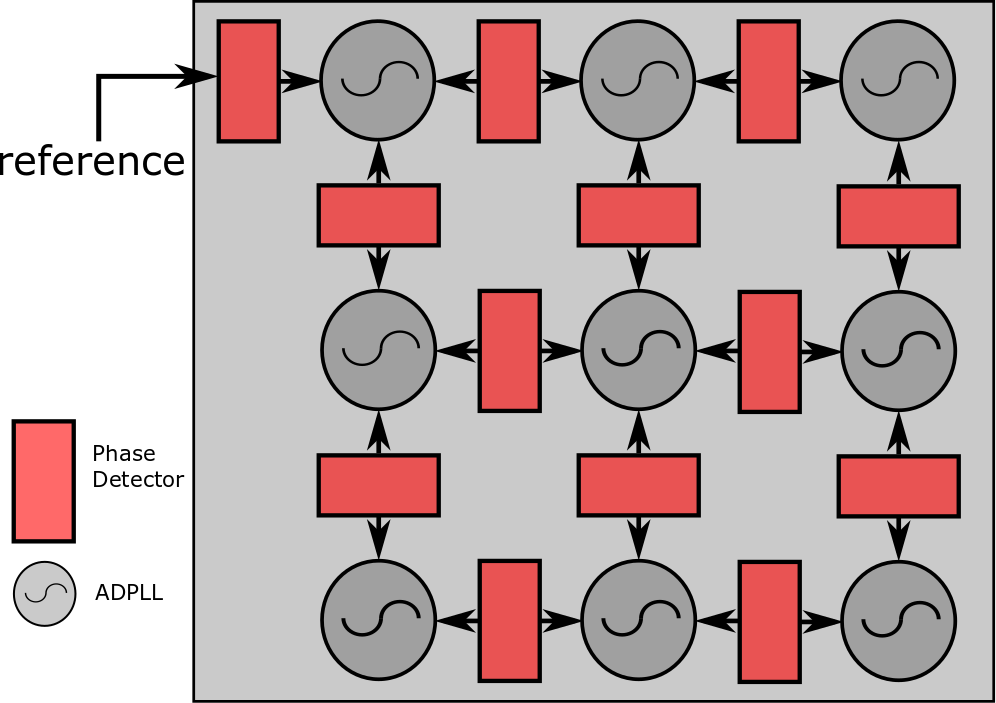
\includegraphics[width=0.25\textwidth]{adpll_network}
	\caption{ADPLL Network Architecture.}
	\label{fig:adpll_network}
	\vspace{0.5cm}
	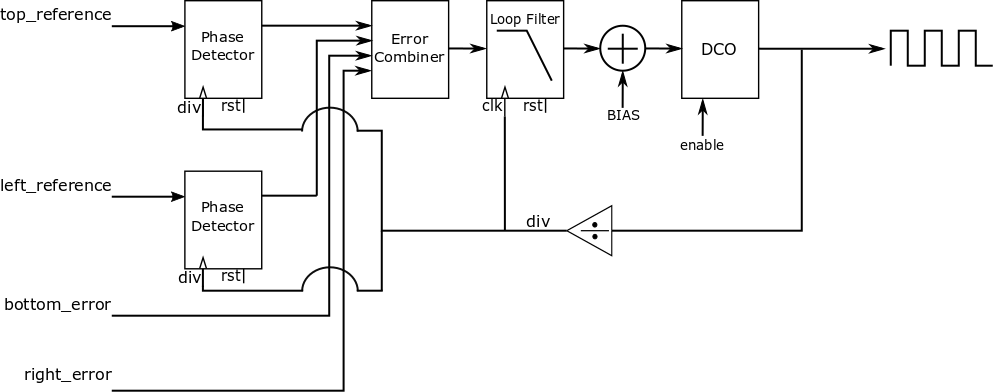
\includegraphics[width=0.4\textwidth]{dist_adpll}
	\caption{Distributed ADPLL Design.}
	\label{fig:adpll_base}
\end{figure}
 Figure \ref{fig:adpll_base} demonstrates the ADPLL design used in this paper.


\newpage
\bibliography{conf.bib} 
\bibliographystyle{IEEEtran}

\end{document}


